% Generated by ASTES Journal Editorial Team
\documentclass{article} %%% use \documentstyle for old LaTeX compilers
\usepackage{geometry}
 \geometry{
 a4paper,
 total={170mm,257mm},
 left=20mm,
 top=20mm,
 }

\usepackage[english]{babel} %%% 'french', 'german', 'spanish', 'danish', etc.
\usepackage{amssymb}
\usepackage{amsmath}
\usepackage{multirow}
\usepackage{txfonts}
\usepackage{multicol}
\usepackage{booktabs}
\usepackage{mathdots}
\usepackage[classicReIm]{kpfonts}
\usepackage{graphicx} %%% use 'pdftex' instead of 'dvips' for PDF output
\usepackage{fancyhdr}
\usepackage{hyperref}
\usepackage{float}
\usepackage{microtype}
\usepackage{subcaption}
\usepackage[justification=centering]{caption}
\usepackage{enumitem}
\pagestyle{fancy}



%Paste this code in page 1
\fancyhead{}
\fancyhead[C]{ }
\renewcommand{\headrulewidth}{0pt }
\fancyfoot{}
\fancyfoot[L]{\href{http://www.astesj.com}{www.astesj.com}}
\fancyfoot[R]{\thepage}
%%%%%%%%%%%%%%%%%%%%%

% You can include more LaTeX packages here 

\makeatletter
\def\@xfootnote[#1]{%
  \protected@xdef\@thefnmark{#1}%
  \@footnotemark\@footnotetext}
\makeatother


\begin{document}

%\selectlanguage{english} %%% remove comment delimiter ('%') and select language if required



\begin{tabular}{p{1in}p{3.8in}p{1.2in}}  
\hspace{-1cm}
\noindent
\begin{tabular}{c}  
\includegraphics[width=2.9cm]{images/ASTES_Logo.jpg}\end{tabular} 	& \centering \textit{Advances in Science, Technology and Engineering Systems Journal \newline Vol. 3, No. 3, XX-YY (2018)} \\   \href{http://www.astesj.com}{www.astesj.com}  
	& \vspace{-0.6cm}  \rule{1.2in}{0.5pt} \vspace{-0.2cm} \newline \centering  \textbf{ ASTES Journal \newline ISSN: 2415-6698} \newline \rule{1.2in}{0.5pt} 
\end{tabular}


\vspace{1.8cm}






\noindent  \textbf{ \LARGE{\setlength\itemsep{0pt}Automatize landmarks setting on Species morphometry using Deep Neural Networks}}

\vspace{0.2cm}

Van-Linh Le\footnote[*]{Corresponding Author Name, Address, Contact No \& Email}${}^{,1,2}$, Marie Beurton-Aimar${}^{1}$, Akka Zemmari${}^{1}$, Nicolas Parisey${}^{3}$

\vspace{0.2cm}
 \textit{${}^{1}$LaBRI-CNRS 5800, University of Bordeaux, 33400, France}

\vspace{0.2cm}
\textit{${}^{2}$ITDLU, Dalat University, 670000, Vietnam}

\vspace{0.2cm}
 \textit{${}^{3}$IGEPP, INRA-1349, 35653, France}

\vspace{0.3cm}

\begin{tabular}{p{1.7in} p{0.1in} p{4.1in} }
A R T I C L E  I N F O &  & A B S T R A C T \\ 
 \cline{1-1}  \cline{3-3} \setlength\itemsep{0pt} \vspace{-0.1cm}
\textit{Article history:\newline Received: \newline Accepted:  \newline Online:  \rule{1.78in}{0.5pt} Keywords: \newline Landmarks\newline Morphometry setting\newline Deep learning\newline Convolutional neural networks} \newline \newline  & & \vspace{-0.1cm} \textit{
Morphometry landmarks are known as one of the
approaches to analyze the characteristics of organisms. Finding
landmarks setting can give to biologists a comprehensive description of the organism. In this study, we propose a convolutional
neural network (CNN) to predict the landmarks on biological's species.
The network is designed as a combination of the ``elementary blocks" including a convolutional layer, a maximum pooling layer, and a dropout layer.
After training with a set of manually landmarks dataset, 
it has been used to predict the morphometric landmarks on biological images automatically.
The network has been checked by applying two scenarios: training from scratch and fine-tuning.
The predicted landmarks have been evaluated by comparing with the coordinates of manual landmarks which have been provided by the biologists.
 The network model is implemented by Python on
Lasagne framework. This paper is an extension of work originally presented in \textbf{2018 1st International Conference on Multimedia Analysis and Pattern Recognition (MAPR)}.}\\
 \cline{1-1}  \cline{3-3}
\end{tabular}


\vspace{0.3cm}

\begin{multicols}{2}



\section{ Introduction}
Morphometry analysis refers to measure the topography of an object, for example, its shape and its size. Biologists work with several parameters from organisms such as lengths, widths, masses, angles,... to analyze the interactions between environment and organisms development. Besides the traditional information, landmarks (or points of interest in the image) are known as one of the characteristics to analyze the shape. Instead of collecting all information, the shape is determined by a finite set of points, called landmarks. They store important information about the shape of the object, \textit{for example}, the corners of the human mouth are a kind of landmarks. Mostly, the landmarks are along the outline of the object but in some special cases, it could be defined inside the anatomical part, \textit{i.e} the landmarks on Drosophila wings are the intersection of veins on fly wings, but the landmarks on pronotum can be located at the shape edge or inside the pronotum. In our study, the morphometric landmarks are specific points defined by biologists. They are used in many biological studyings. Currently, the landmarks are set manually by the entomologist, the operation are time-consuming and difficult to reproduce when the operators change. Therefore, a method that gives automatic location of landmarks could have a lot of interest.

In this study, we work on a dataset including the images of collecting from $293$ beetles in Brittany lands. All the images are presented in RGB color with two dimensions. For each beetle, the biologists took images of five parts: \textit{left and right mandibles, head, body, and pronotum} (Figure \ref{fig1}). For each part, a set of manual landmarks has been positioned by an entomologist.

In the concept of automatically landmarks setting, image processing is usually the first choice to apply. This is a process that we apply a set of algorithms (in image processing) to extract and to analyse the object of interest. In which, segmentation is most often the first and the most important step. This task remains a bottleneck to compute features of an image. In some cases, the object of interest is easy to extract and can be analyzed with the help of a lot of very well-known image analysis procedures. Like previous study \cite{le2017maelab}, we have analyzed two parts beetle mandibles (Figure \ref{figsub01} and Figure\ref{figsub02}). These parts are pretty easy to segment (enough good quality for our goals). In that work, we have applied a set of algorithms based on the combination of principal component analysis \cite{shlens2014tutorial} and SIFT descriptor \cite{lowe2004distinctive}. 
Unfortunately, this method is irrelevant with the case of the images that are not precise or difficult to segment, \textit{i.e.} pronotum images. So, the remain question of how to predict the landmarks on the images like the pronotum images? This is the reason why we have turned to a way of analyzing images without need for a segmentation step. So, the next step has been to work with the prontoum images (Figure \ref{figsub05}). For each pronotum image, a set of 8 manual landmarks have been set by the biologists (Figure \ref{figmlm}). They are considered as the ground truth to evaluate the predicted landmarks by our method.

\begin{figure}[H]
    \centering
    \begin{subfigure}[t]{0.23\textwidth}
        \centering
        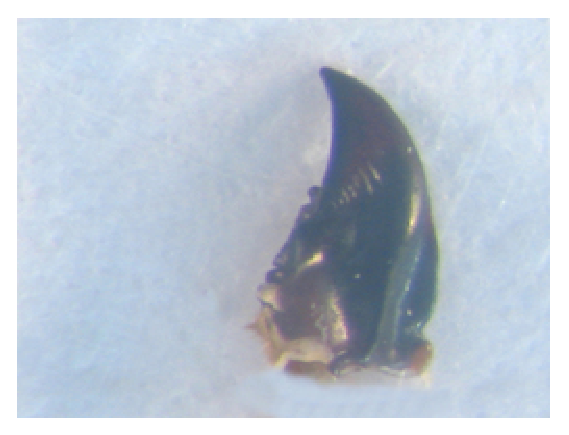
\includegraphics[height=1in]{images/md19.eps}
        \caption{\footnotesize{Right mandible}}
        \label{figsub01}
    \end{subfigure}%
    ~ 
    \begin{subfigure}[t]{0.23\textwidth}
        \centering
        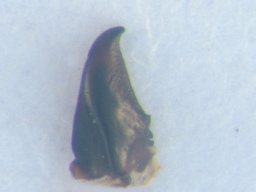
\includegraphics[height=1in]{images/mg019.JPG}
        \caption{\footnotesize{Left mandible}}
        \label{figsub02}
    \end{subfigure}~\\
    \begin{subfigure}[t]{0.23\textwidth}
        \centering
        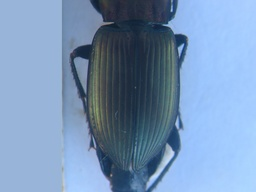
\includegraphics[height=1in]{images/elytre107.JPG}
        \caption{\footnotesize{Elytra}}
        \label{figsub03}
    \end{subfigure}%
    ~ 
    \begin{subfigure}[t]{0.23\textwidth}
        \centering
        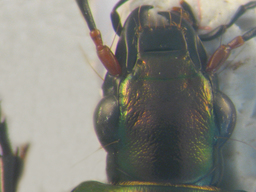
\includegraphics[height=1in]{images/tete081.JPG}
        \caption{\footnotesize{Head}}
        \label{figsub04}
    \end{subfigure}~\\
    \begin{subfigure}[t]{0.23\textwidth}
        \centering
        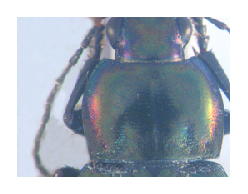
\includegraphics[height=1in]{images/prono60.eps}
        \caption{\footnotesize{Pronotum/thorax}}
        \label{figsub05}
    \end{subfigure}
    \caption{\footnotesize{The anatomical parts of beetle}}
    \label{fig1}
\end{figure}

To achieve the landmarks prediction, this work introduces a method for this automatic detection of the landmarks on pronotum images. The main idea consists on design and train of a CNN \cite{lecun2010convolutional} with a set of manual landmarks. In the first stage, the network has been trained from scratch on the dataset of pronotum images from the first model. In the second step, the training has been modified to improve the quality of prediction by including the fine-tuning\cite{torrey2009transfer} step. The network has been implemented by using Python on Lasagne library \cite{lasagne}.

\begin{figure}[H]
	\centering
	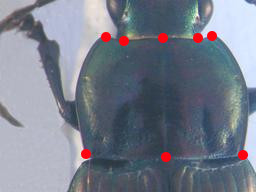
\includegraphics[height=1.5in]{images/pronotum.jpg}
	\caption{\footnotesize{A pronotum image with its eight manual landmarks}}
	\label{figmlm}
\end{figure}

The rests of the article is organized as follows. In the next of two sections, we give a briefly overview of the related works on automatically landmarking and a shortly about the CNN. After that, in Section \ref{SecApp}, we apply the CNN to predict the landmarks on pronotum images: Firstly, we describe the processes that we have used to augment the dataset (Section \ref{Secdataaug}). Secondly, in the Section \ref{SecArch}, we present the architecture of the proposed network and its parameters also. Finally, we give the first results of the model in Section \ref{Secfirstrs}. From the first results, we present the steps of fine-tuning procedure to improve the result in Section \ref{secimproving}. Finally, we conclude the article with a discussion of future works in Section \ref{Secconclusion}.

\section{Related works}
A landmark is a specific point that may contain useful information. For example, the tip of the nose or the corners of the mouth are landmarks on human face \cite{sun2013deep}. Under image processing point of view, when we want to extract the feature from the image, we can consider two kinds of cases: the object of interest can be segmented or not. Setting landmarks can not be achieved in the same way depending on which situation we are. When segmentation can be applied, Lowe et al. \cite{lowe2004distinctive} have proposed SIFT method to find the corresponding keypoints in the 2D images. From the detected keypoints, the method is able to match two images. Palaniswamy et al. \cite{palaniswamy2010automatic} have proposed a method based on probabilistic Hough Transform to automatically locate the landmarks in digital images of Drosophila wings. In previous work \cite{le2017maelab}, we have proposed a method which have been extended from Palaniswamy's method, to determine landmarks on mandibles of beetles. The mandibles of beetle have the simple shape and easy to segment. We have obtained good enough results about determining the landmarks automatically on mandibles. Unfortunately, after several tests, we have had to conclude that this way does not provide good results with the pronotum images because the pronotum segmentation has too many noises.

In recent years, deep learning is known as a solution for many tasks in different topics. In image analysis domain, using deep learning, namely CNN, to determine the landmarks on 2D images has achieved better results even if the images that can not segment. Yi Sun et al. \cite{sun2013deep} have proposed cascaded CNNs to predict the facial points of interest on the human face.
Zhanpeng Zhang et al. \cite{zhang2014facial} proposed a \textit{Tasks-Constrained Deep Convolutional Network} to optimize facial landmarks detection. Their model determines the facial landmarks with a set of related tasks such as head pose estimation, gender classification, age estimation, face recognition, or facial attribute inference. Cintas et al. \cite{cintas2016automatic} has introduced a network to predict the landmarks on human ears. After training, the network has the ability to predict 45 landmarks on human ears. In this way, we have applied CNN computing to work with pronotum landmarks.

\section{Convolutional neural networks}
Deep learning models are coming from the machine learning theory. They have been introduced in the middle of previous century for artificial intelligence applications but they encounter several problems to take real-world cases. Fortunately, the improvement of computing capacities both in memory size and computing time with GPU programming has opened the new perspective for deep learning. 

Deep learning allows computational model composed of multiple processing layers to learn representations of data with multiple levels of abstraction \cite{lecun2015deep}. Each layer extracts the representation of the input data from the previous layer and computes a new representation for the next layer. In the hierarchy of a model, higher layers of representation enlarge aspects of the input that is important for discrimination and suppress irrelevant variations. Each level of representations is corresponding to the different level of abstraction. During training, it uses gradient descent optimization method to update the learnable parameters via backpropagation. The development of deep learning opens promise results for well-known problems artificial intelligence on high dimensional data, therefore applicable to many domains: image recognition and classification \cite{krizhevsky2012imagenet,ciregan2012multi,szegedy2015going}, speech recognition \cite{mikolov2011strategies,hinton2012deep,sainath2013deep}, question answering \cite{bordes2014question}, language translation \cite{sutskever2014sequence, jean2014using}, and recognition \cite{li2015convolutional, tompson2014joint}.

A CNN consists of a number of connected layers. The layers of a CNN has neurons arranged in three dimensions: \textit{width, height, and depth} with learnable parameters. Figure \ref{figconvarc} shows a classical example of CNN. It is a pipeline of usual layers: convolutional layers (CONV), pooling layers (POOLING), dropout layers (DROPOUT), and full-connected layers (FC).

\begin{figure}[H]
	\centerline{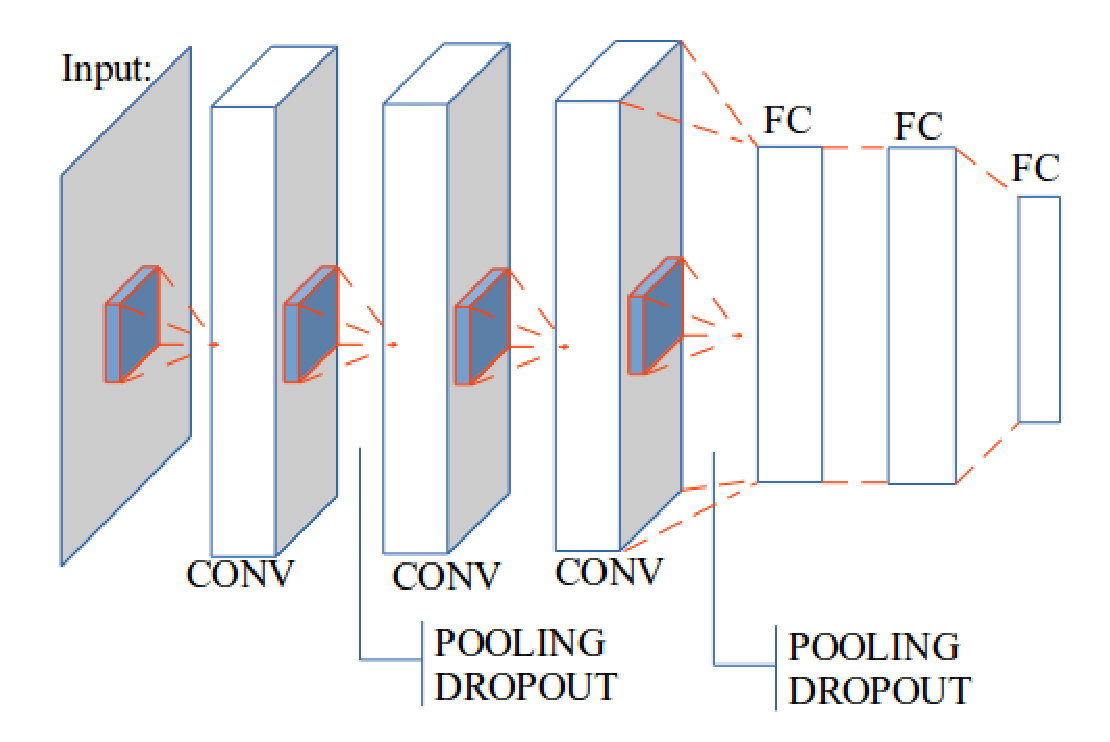
\includegraphics[height=1.8in]{images/convarc.eps}}
	\caption{\footnotesize{An example of usual convolutional neural network}}
	\label{figconvarc}
\end{figure}

A \textit{convolutional} layer computes a dot product between its weights and a small region in the input. At the output, the results of connected local regions are combined. Convolution layer uses a set of learnable filters as parameters. Each filter is small spatially but extends the depth of the input. \textit{Pooling} layer is used to down-sampling the input, to reduce the computational cost in remaining layers, and to control overfit. \textit{Dropout} layer refers to dropping out units in the network. Dropping a unit out means temporarily removing it from the network, along with all its incoming and outgoing connections. \textit{Full connected} layer refers to the output of the network. The number of outputs of the last full-connected layer are corresponding to the number of predicted values.

From the beginning of deep learning until now, many deep learning frameworks have been developed.
These frameworks help the users to design their application by re-using already proposed network architectures. Almost frameworks are open source. According to the written programming languages, the frameworks can be separated into two main groups: C++, \textit{such as Caffe, Deeplearning4j, Microsoft Cognitive Toolkit} and Python \textit{i.e Keras, Theano, PyTorch}. Another framework exists using more confidential languages as \textit{Lua}.

Theano \cite{theanoframework} is an open source framework developed by the machine learning group at the University of $Montr\acute{e}al$. It is a Python library that allows to define, to optimize and to evaluate mathematical expressions relating multi-dimensional arrays efficiently by using a Numpy package. Theano supports compilation on either CPU or GPU architectures. Lasagne \cite{lasagne} is a lightweight library in Theano. It allows to build and to train the neural networks. In this work, we have used Lasagne to implement the proposed neural network. Recently, Theano has been stopped to develop but its community is still large. The networks which have been designed by Theano are still useful and efficient in deep learning area.
\section{Application to landmarks identification}
\label{SecApp}
In the previous sections, we have presented an overview of automatic landmarks setting and CNN. In the first of this section, we describe the process to augment the dataset which is considered as a little bit small to apply deep learning. Then, we present the designing the processes of the network architecture that we use to predict the landmarks on pronotum images.

\subsection{Data augmentation}
\label{Secdataaug}
In deep learning, data are one of the most important elements besides the network architecture. When we train a network with a lot of parameters, we need to show the network a proportional amount of example to get the best performance. For example, VGGNet \cite{.} have been trained on a dataset including $1.2$ million images to classify them into $1000$ classes. However, data for deep learning problems are not always available in practice. In some cases, the number of images is very limited. So,
we need the techniques to enlarge the data that we have. For instance, to get more data, we just need to make minor alterations to an exsting dataset such as flips or translation or rotation, \ldots. Of course, the network will think these are distinct inputs. More specifically, a CNN can be invariant to translation, viewpoint, or illumination. Come back with our problem, the main purpose is to predict the landmarks on pronotum images. If we apply the usual augmentation methods, we need to re-point the manual landmarks before using. Additional, our model has been designed to work on the input of a channel. So, we have decided to work on the channels of the image to augment the dataset.

Our images come from a collection of 293 beetles from Brittany lands. All the images are taken with the same camera under same conditions with a $3264 \times 2448$ resolutions. For each specific part, a set of manual landmarks has been determined by biologists. The provided dataset contains 293 pronotum images, each image with 8 landmarks provided by biologists (Figure \ref{figmlm}). The dataset was split into a training set with 260 images (training and validation) and a testing set of 33 images. During the training, the network learned the information through a pair of \textit{image and manual landmarks} in the training set. At the testing stage, the image without landmarks is given to the trained network and the predicted landmarks coordinates will be given as output. Figure \ref{figmlm} shows an example of pronotum image with its manual landmarks.

In some published networks \cite{krizhevsky2012imagenet, sun2013deep, cintas2016automatic}, the maximum size of the inputs is not over 256 pixels. In our case, the resolution of the image is large, it becomes a difficulty for the computing. Before training and testing, the images are down-sampling to a new resolution of $256 \times 192$. Obviously, the landmark coordinates of the image are also scaled to suit their new resolution. Then, we have applied two another procedures to increase the number of images in the dataset.

%In CNN, the network usually has a large number of learnable parameters. In addition, if the dataset is limited, the result, that we obtain, will have a large errors between the training and the testing processes. It means that the over-fitting had occured during the training process. In our case, the dataset is limited in $293$ pronotum images. This number is very small in the context of deep learning. Therefore, we need to enlarge the size of the dataset. In image processing, we usually apply transform procedure (i.e rotation, translation,...) to generate a new image but the analysis of image by CNN is most often translation and rotation invariant. Therefore, we have applied two another procedures to increase the number of images in the dataset.

The first procedure has been applied to change the value of each channel in the original image. According to this, a constant is added to a channel of RGB image and for each time, we just change the value of one of three channels. For example, from an original RGB image, if we add a constant $c = 10$ to the red channel, we will obtain a new image with a different profile histogram. By this way, we can generate three new RGB images from one RGB image. Figure \ref{figpronotum} presents $3$ new versions of an original image by adding a value $c = 10$ to each channel for each time.

\begin{figure}[H]
	\centerline{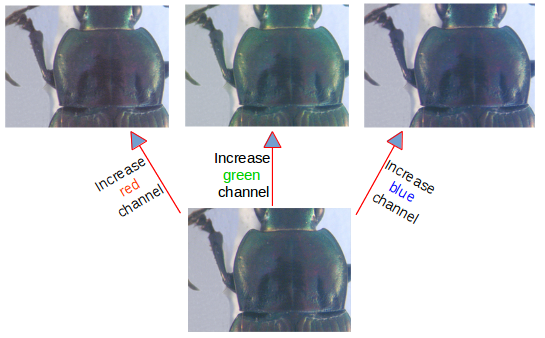
\includegraphics[height=1.9in]{images/inc_channels.png}}
	\caption{\footnotesize{A constant (c=10) has been added to each channel of an original image for each time}}
	\label{figpronotum}
\end{figure}

The second procedure splits the channels of RGB images. It means that we separate the channels of RGB into three gray-scale images. Figure \ref{figpronotum2} shows the values at three individual channels of an image. At the end, we can generate six versions of original image, the total number of images used to train and validate is $260 \times 7 = 1820$ images (six versions and original image). The dataset that has been used for training and validation is split randomly by a ratio (training: $60\%$, validation: $40\%$) that has been set during the network setup.

\begin{figure}[H]
	\centerline{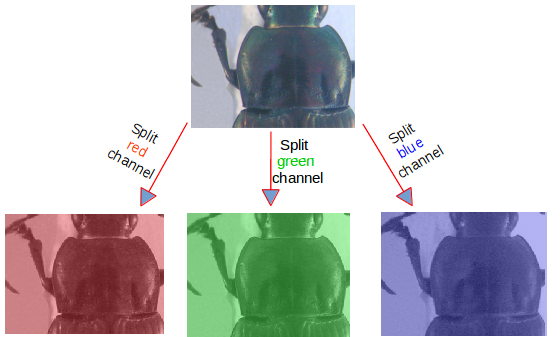
\includegraphics[height=1.9in]{images/sp_channels.png}}
	\caption{\footnotesize{The individual channels have been extracted from an original image}}
	\label{figpronotum2}
\end{figure}

In practical, when we work with CNN, convergence is usually faster if the average of each input variable over the training set is close to zero. Moreover, when the input is set closed with zero, it will be more suitable with the sigmoid activation function \cite{lecun2012efficient}. According to \cite{lecun2012efficient}, the brightness of the image is normalized to $[0,1]$, instead of $[0,255]$ and the coordinates of the landmarks are normalized to $[-1,1]$, instead of $[0,256]$ and $[0,192]$ before to be giving to the network.
\subsection{Network architecture}
\label{SecArch}
Three different networks models have been proposed and trained to perform the best architecture for automatically landmarking predictions. They receive the same input of $1 \times 256 \times 192$ to train but they have different number of layers. In this section, we introduce the architectures of the networks and the process to improve the architecture from the beginning of designing.

\subsubsection{The first networks}
The designing begins with some basically layers in CNN. The network consists on three repeated-structure of a convolutional layer followed by a maximum pooling layer. Figure \ref{figarch0} shows the architecture of the first model which is a very classical one. The depth of convolutional layers increases from $32, 64,$ and $128$ with different sizes of the filter kernels: $3 \times 3$, $2 \times 2$, and $2 \times 2$. All the kernels of pooling layers have the same size of $2 \times 2$. The kernel sizes are classical as the literature. At the end, three full connected layers have been added to the network. The outputs of the full connected layers are $500, 500,$ and $16$, respectively. The output of the last full-connected layer corresponds to 8 landmarks ($x$ and $y$ coordinates) which we would like to predict. The training result shows that the architecture of this model provides overfitting and so is not good enough to solve the problem.

\begin{figure}[H]
	\centerline{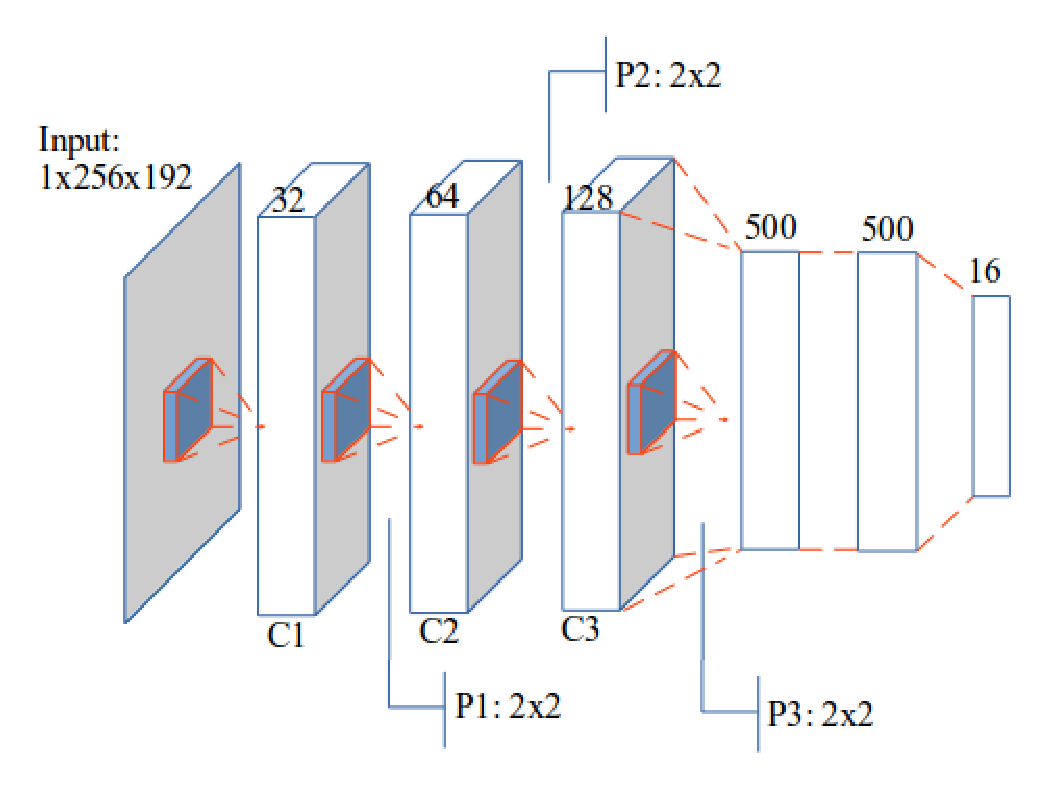
\includegraphics[height=2in]{images/architecture1.eps}}
	\caption{\footnotesize{The architecture of the first network}}
	\label{figarch0}
\end{figure}

The second network has been improved from the first architecture by modifying the output the full-connected layers from $500$ to $1000$. The goal of this change is to have more connections to all activations in the previous layer and we would like to prevent the overfitting but the result did not lead to better performances.

In the next step to lead to the performance of the network, instead of changing the parameters, we have decided to add some layers into the model. Srivastava et al. \cite{srivastava2014dropout} suggest to use dropout sequence to correct overfitting artifacts. This is considered as the good solution to prevent the overfitting. The idea of dropout is to randomly drop units from the neural network during training. It prevents units from co-adapting too much. During training, dropout samples are done from an exponential number of different ``thinned" network. At test times, it is easy to approximate the effect of averaging the prediction of all thinned networks by simply using a single unthinned network with smaller weights. This significantly reduces overfitting and gives major improvements over other regularization methods \cite{srivastava2014dropout}. After several testing, we have decided to keep the concept of \textit{``elementary blocks"} to compose and to create the network.

\subsubsection{Elementary block and selected architecture}
An \textit{elementary block} is defined as a sequence of
convolution (\textit{$C_i$}), pooling (\textit{$P_i$}) and dropout(\textit{$D_i$}) layers that can be repeated several
times before to achieve the computation with the full-connected
layers. For our purpose, we have assembled $3$ \textit{elementary
  blocks} in our model (see Fig.\ref{figarch}). The parameters for
each layer are as below, the list of values follows the order of
\textit{elementary blocks}:

\begin{itemize}[nosep,label=\footnotesize$\bullet$]

\item CONV layers:
		\begin{itemize}[nosep]
			\item Number of filters: $32, 64,$ and $128$,
			\item Kernel filters size: $(3 \times 3), (2 \times 2),$ and $(2 \times 2)$,
			\item Stride values: $1, 1, 1$,
			\item No padding is used for CONV layers.
		\end{itemize}			
	\item POOL layers:
		\begin{itemize}[nosep]
			\item Kernel filters size: $(2 \times 2), (2 \times 2),$ and $(2 \times 2)$,
			\item Stride values: $2, 2, 2$.
			\item No padding is used for POOL layers.
		\end{itemize}
	\item DROP layers: 
		\begin{itemize}[nosep]
			\item Probabilities: $0.1, 0.2, $ and $0.3$.
		\end{itemize}
	\end{itemize}
In the last full-connected layers (FC), the parameters are: FC1 output:
$1000$, FC2 output: $1000$, FC3  output: $16$. As usual, a dropout layer is
inserted between FC1 and FC2 with a probability equal to $0.5$.
Actually, we keep the same value for the parameters of the convolutional ($32, 64,$ and $128$), pooling ($3 \times 3$, $2 \times 2$, and $2 \times 2$) and full-connected layers ($1000, 1000,$ and $16$) as the second one.

\begin{figure*}[t]
	\centerline{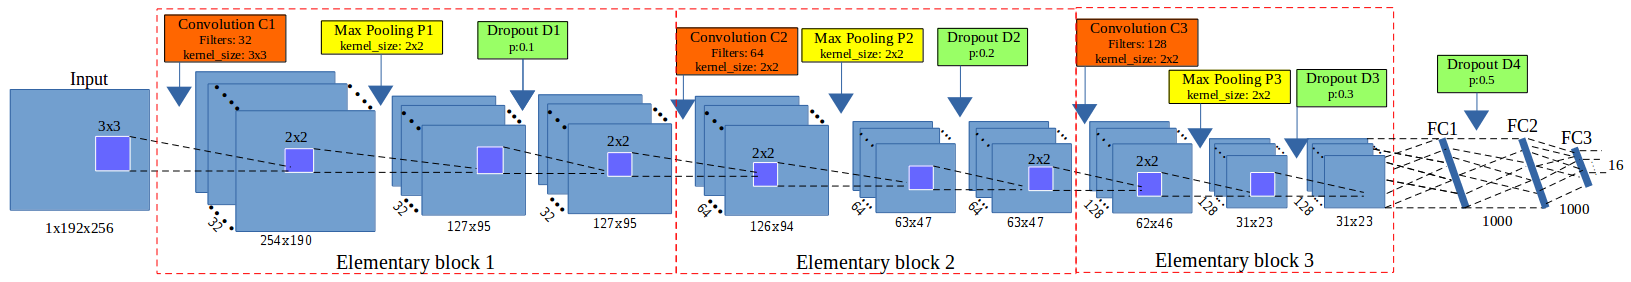
\includegraphics[height=1.1in]{images/arch_model.png}}
	\caption{\footnotesize{The architecture of the last network}}
	\label{figarch}
\end{figure*}

\subsection{Training}
The proposed model has been trained with $1,820$ image in $5000$ epochs\footnote{An epoch is a single pass through the full training set.}. To obtain the predicted landmarks on all images, we have applied cross-validation technique to select the training data in the training process. During the training, the network is designed with a small sharing learning rate and a momentum. As usual, these parameters have been used to perform gradient descent during backward phase to update the parameters of the layers. The value of learning rate and momentum are updated over training time to fit with the remaining number of iterations: the momentum value has been adjusted in a range of $0.9 \rightarrow 0.9999$ and the learning rate value has been adjusted from $0.03$ to $0.00001$. 

The implementation of this architecture used Python on Lasagne framework \cite{lasagne} which allows to train the network on GPU. The training process took around 3 hours using NVIDIA TITAN X cards. The design of the network is available on GitHub\footnote{It is freely obtained by request the authors.}.

\subsection{First results}
\label{Secfirstrs}
Usually, the first performance of a CNN is appreciated from the loss values in training and validation steps. In the context of deep learning, landmark prediction can be seen as a regression problem. Therefore, to evaluate the results, we have used root mean square error (RMSE) to compute the accuracy of the implemented architecture. 

Figure \ref{figloss1} and \ref{figloss} show the training errors and the validation errors of a training time on the first and the third model, respectively. The blue curves present RMSE on training dataset, the green curves present the validation errors. Clearly, the overfitting has appeared in the first model. In Figure \ref{figloss1}, we can see that if the training is able to decrease with the number of epochs, it is not the case of validation loss. At the opposite in the third model, we can see some different values for the two losses at the beginning but after several epochs, these values become more proximate and the overfitting problem has been solved.

\begin{figure}[H]
	\centerline{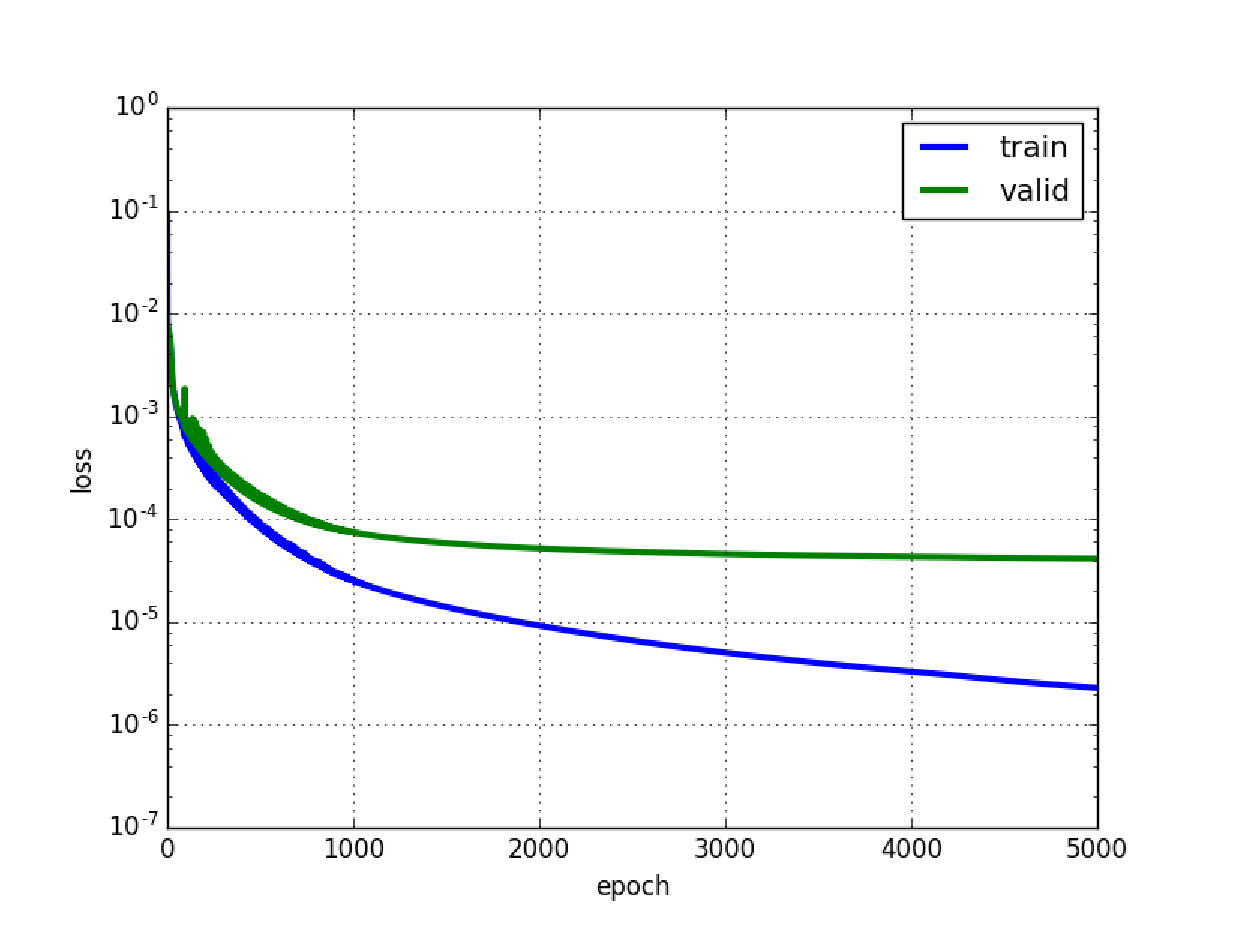
\includegraphics[height=2.3in]{images/loss_model_1.eps}}
	\caption{\footnotesize{Learning curves of the first model.}}
	\label{figloss1}
\end{figure}~\\
\begin{figure}[H]
	\centerline{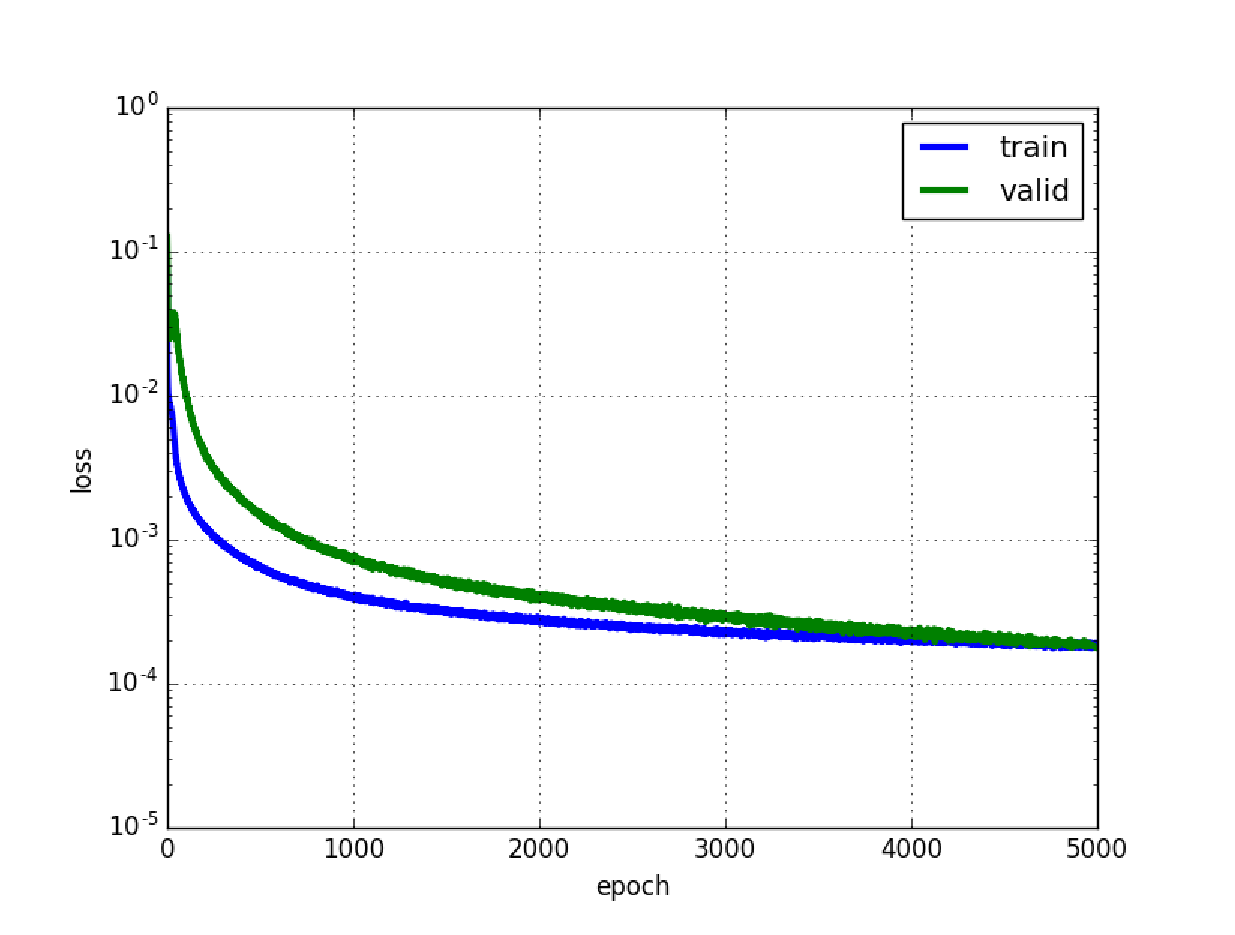
\includegraphics[height=2.3in]{images/loss_v16.eps}}
	\caption{\footnotesize{Learning curves of the last model.}}
	\label{figloss}
\end{figure}

To have the correct view about the predicted landmarks, we would like to evaluate the results in other views by using the manual landmarks coordinates (which have provided by the biologists) as ground truth. Firstly, we have considered the results in a statical point of view. We have computed the quality metric to measure the linear cofficient between the coordinates of predicted and manual landmarks. The scores have been calculated based on $3$ quality metrics: cofficient of determination ($r^2$), explained varicance (EV), and Pearson correlation (using \textit{scikit-learn} \cite{pedregosa2011scikit}) like Cintas et al. \cite{cintas2016automatic} have done. Table. \ref{table1} shows the comparison between our and their scores. From the scores, we can see that the quality of predicted coordinates are very precise.

\begin{table}[H]
	\centering
	\begin{tabular}{|c|p{1cm}|p{1cm}|p{1.5cm}|}
		\hline
		Metric & $\mathbf{r^{2}}$ & \textbf{EV} & \textbf{Pearson} \\ \hline
		Cintas et al & $0.884$ & $0.951$ & $0.976$ \\ \hline
		Our score & $\textbf{0.9952}$ & $\textbf{0.9951}$ & $\textbf{0.9974}$ \\ \hline
	\end{tabular}
	\caption{\footnotesize{The cofficient on the quality metrics}}
	\label{table1}
\end{table}

Then, we have considered the results on the point view of image processing. Figure \ref{figresult1} display the landmarks on the images. The red points are manual landmarks and the yellow points are predicted landmarks. The landmarks in Figure \ref{figsubrs1} are a well-prediction, while they are less accurated in the case of Figure \ref{figsubrs2}.

\begin{figure}[H]
    \centering
    \begin{subfigure}[t]{0.25\textwidth}
        \centering
        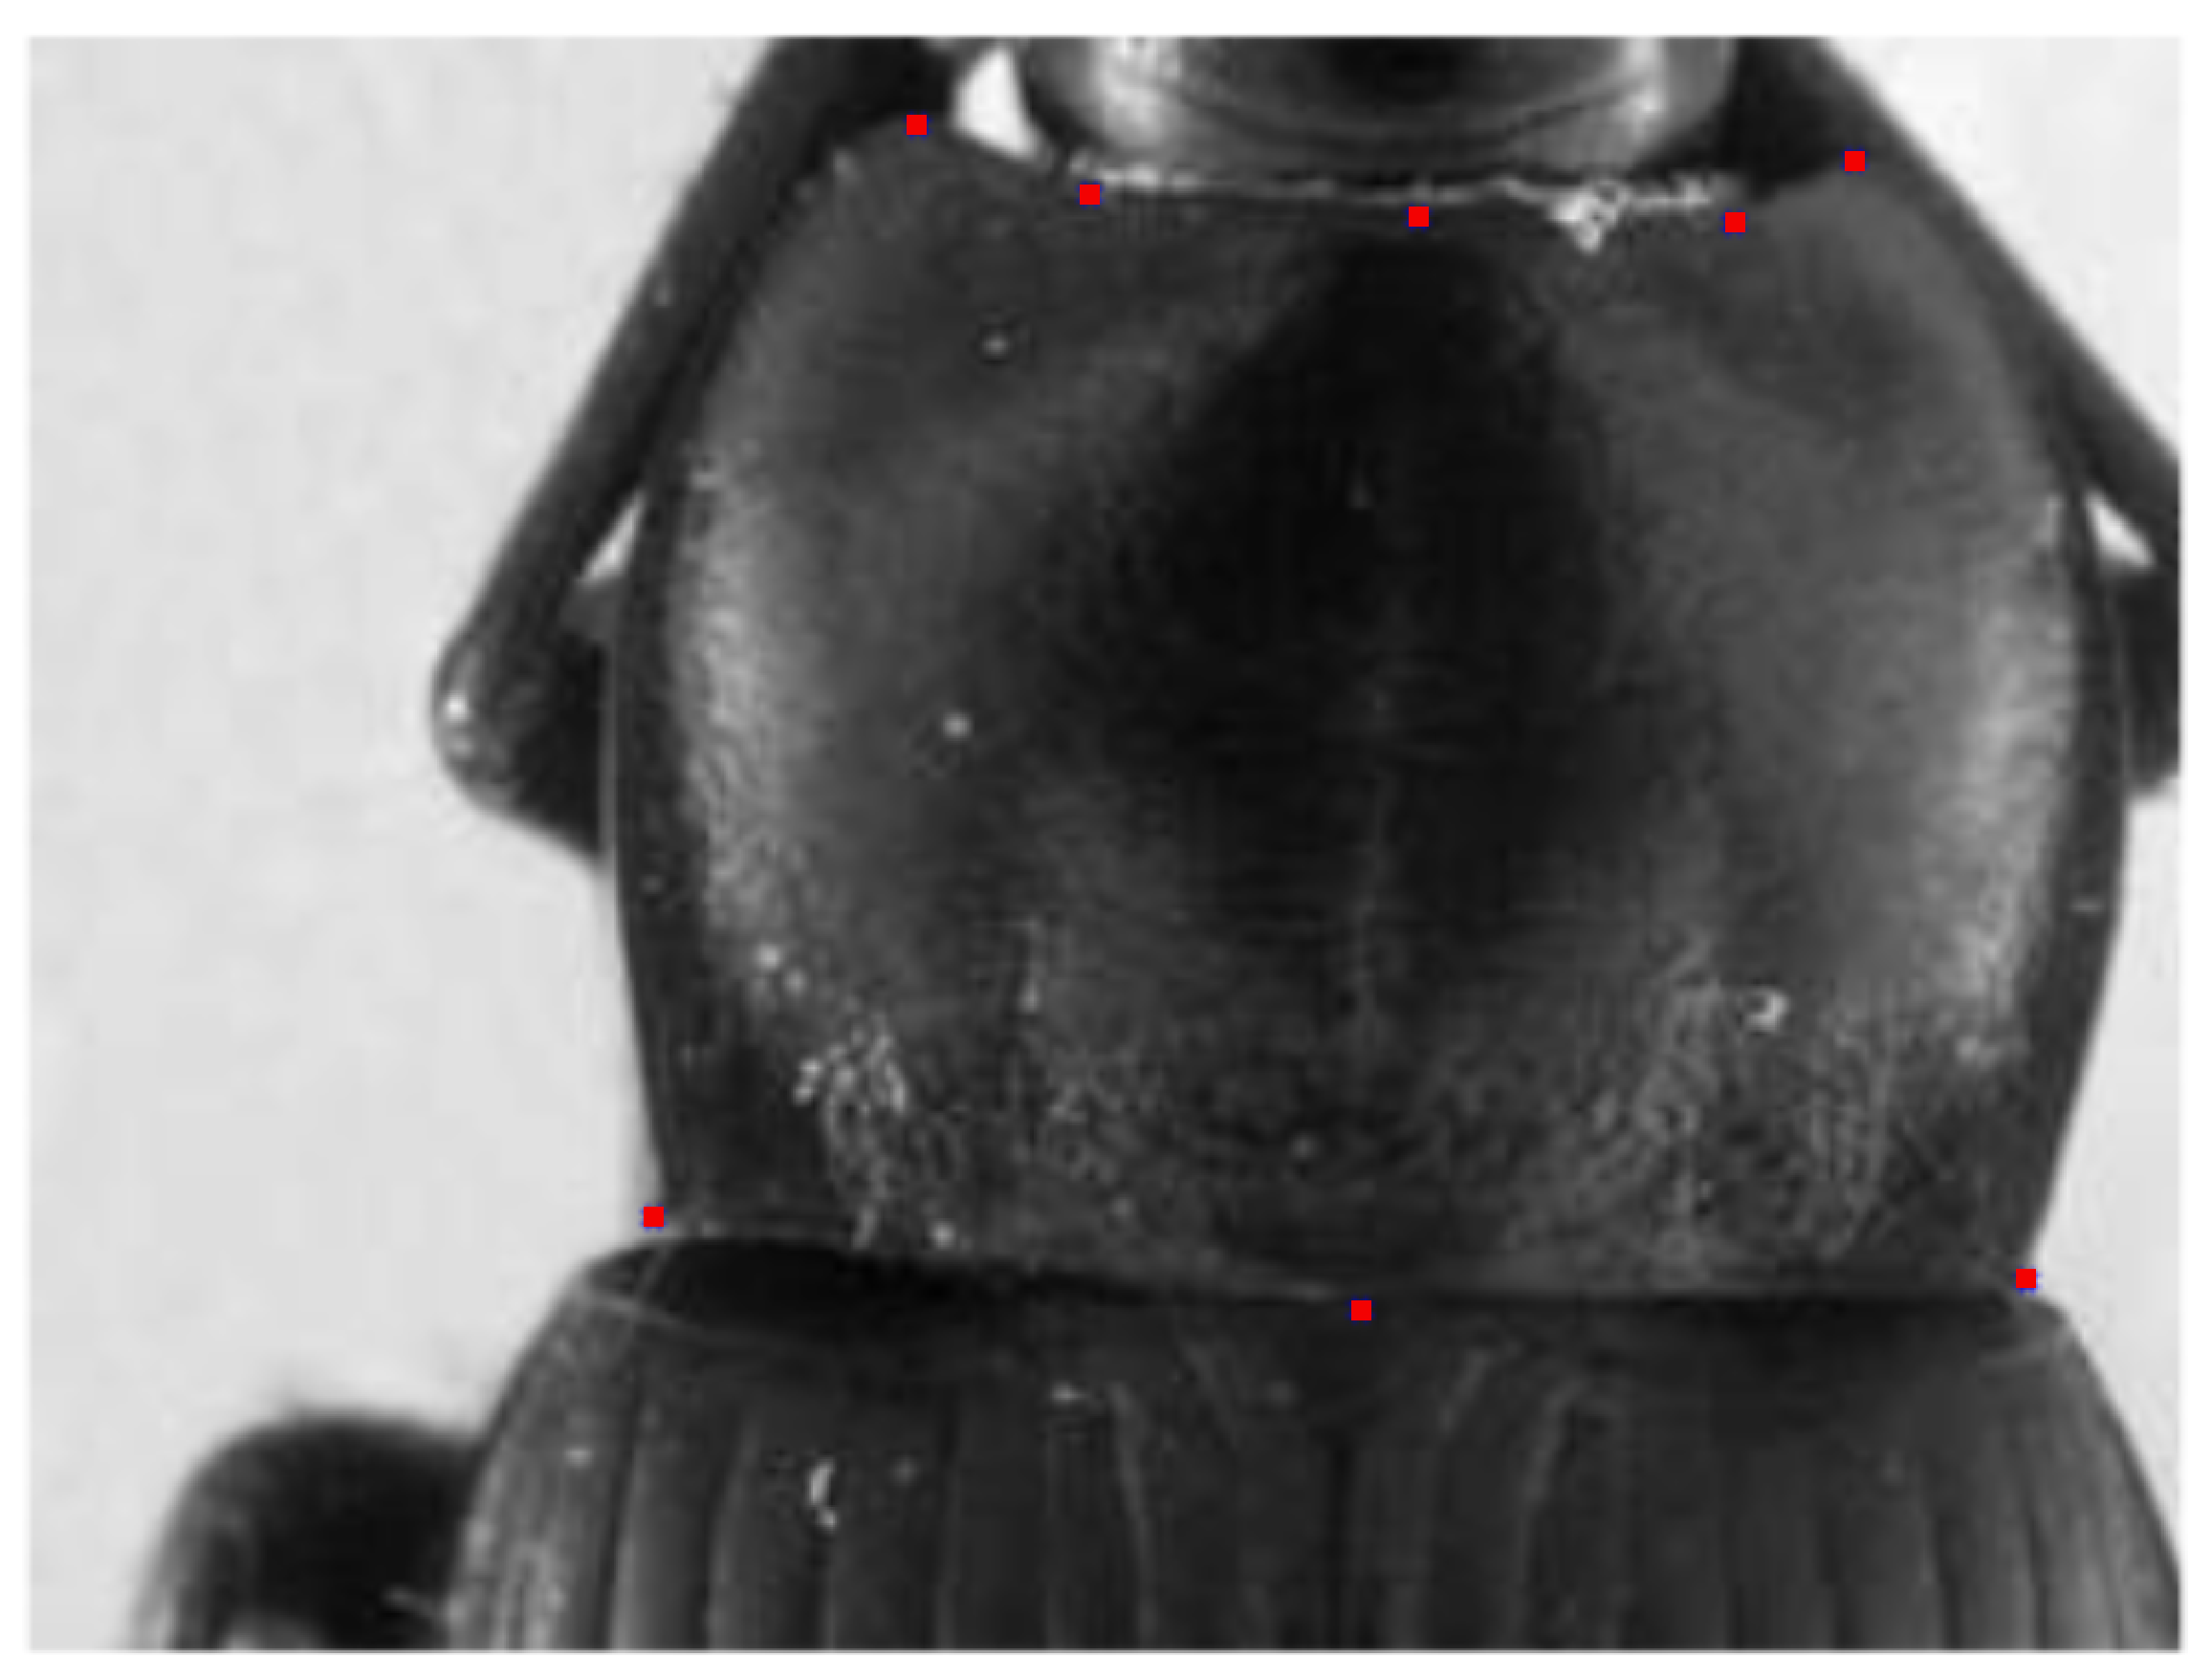
\includegraphics[height=1.2in]{images/plandmark.eps}
        \caption{\footnotesize{Image with well-predicted landmarks}}
        \label{figsubrs1}
    \end{subfigure}%
    ~ 
    \begin{subfigure}[t]{0.25\textwidth}
        \centering
        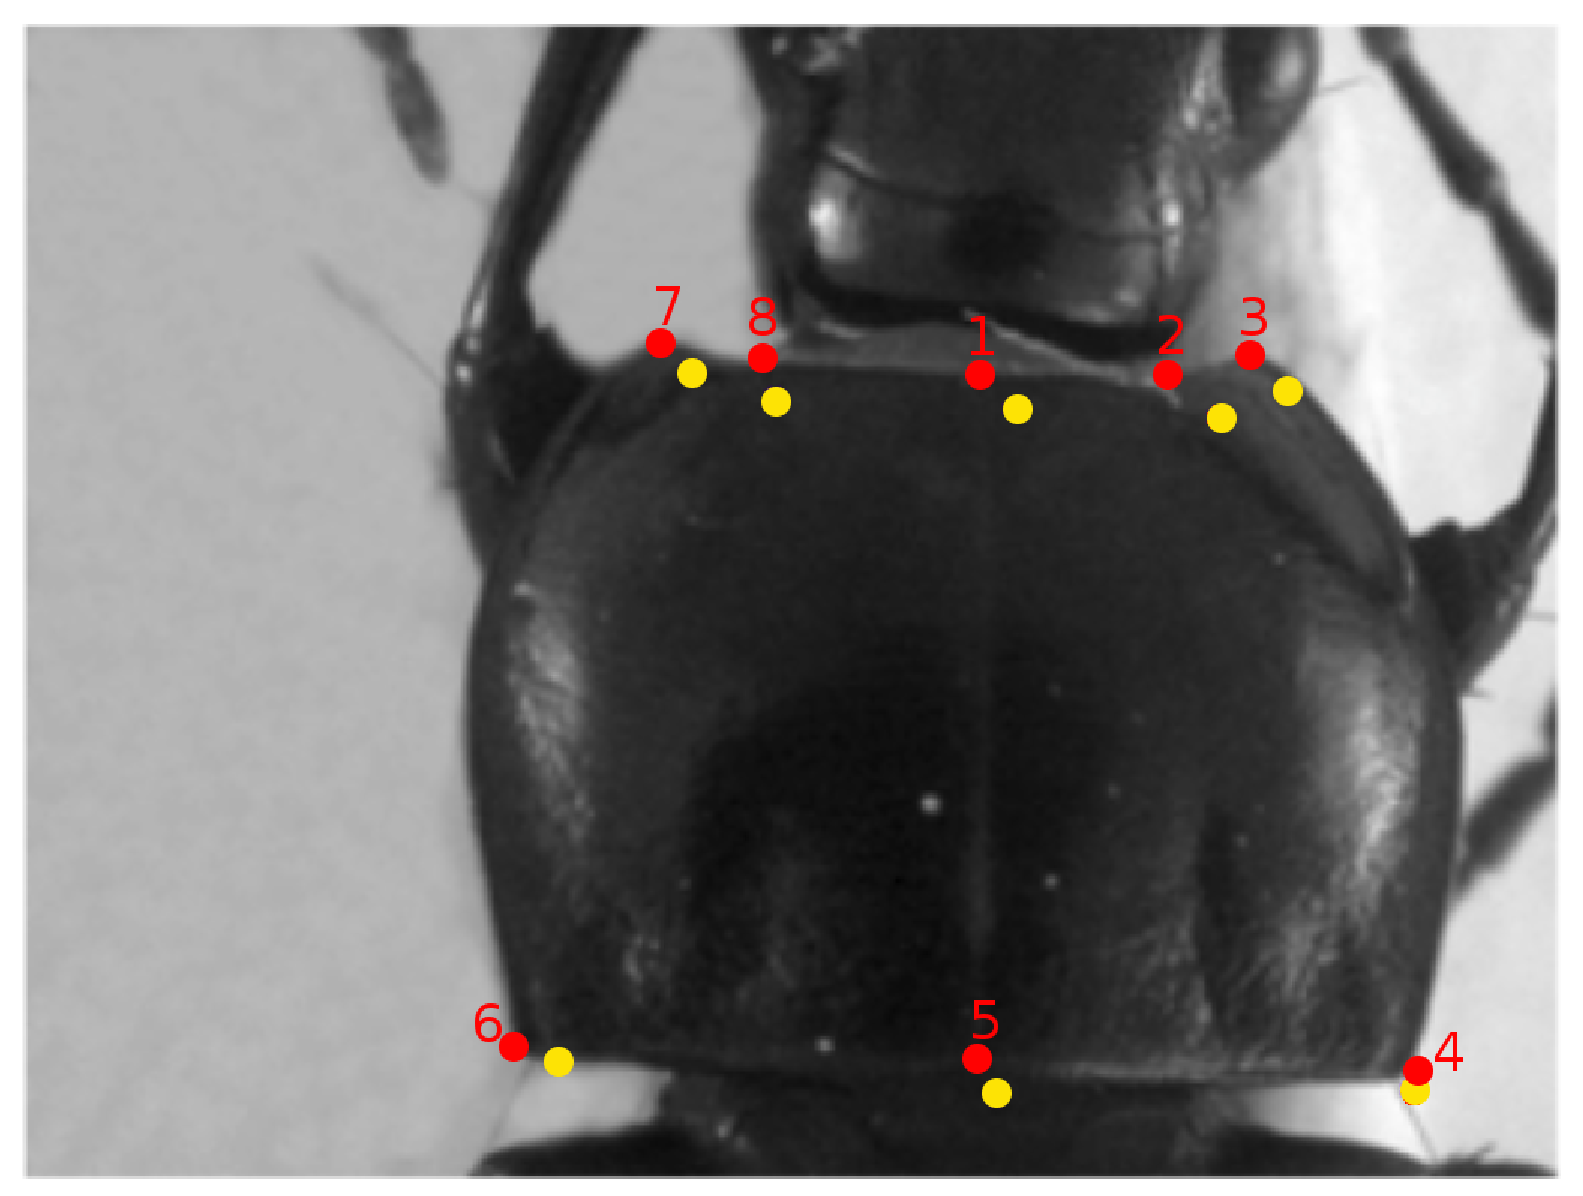
\includegraphics[height=1.2in]{images/plandmark2.eps}
        \caption{\footnotesize{Image with fewer accuracy landmarks}}
        \label{figsubrs2}
    \end{subfigure}
    \caption{\footnotesize{The predicted landmarks on an image in test set (yellow points)}}
    \label{figresult1}
\end{figure}

To have a correct assessment of predicted coordinates, we have calculated the distances between the predicted and corresponding manual landmarks in all images. Then, we have computed the average distance per landmark as presented in Table. \ref{table2}. The minimum distance is around $4$ pixels in the $1^{st}$ landmark, while the worst distance is more than $5$ pixels in the $6^{th}$ landmark. The other distances are approximate $4.5$ pixels.
\begin{table}[H]
	\centering
	\begin{tabular}{|c|c|}
		\hline
		\textbf{$\#$Landmark} & \textbf{Distance} (in pixels) \\ \hline
		1 & 4.002  \\ \hline
		2 & 4.4831 \\ \hline
		3 & 4.2959 \\ \hline
		4 & 4.3865 \\ \hline
		5 & 4.2925 \\ \hline
		6 & 5.3631 \\ \hline
		7 & 4.636 \\ \hline
		8 & 4.9363 \\ \hline
	\end{tabular}	
	\caption{\footnotesize{The average distance per landmark}}
	\label{table2}
\end{table}

In other view, we have computed the standard deviation \cite{bland1996statistics} which is used to quantify the dispersion of a set of distances. For example, Figure \ref{figchartlm1} shows the distribution of the distances on the first landmark of all images. The accuracy based on the distance in each image can be separated into three spaces: the images have the distance less than average value ($4$ pixels): \textbf{56.66$\%$}; the images have the distance from average value to $6.5$ pixels (average distance plus standard deviation): \textbf{$28.33\%$}; and the images have the distance greater than $6.5$ pixels: \textbf{$15.02\%$}. 

\begin{figure}[H]
	\centerline{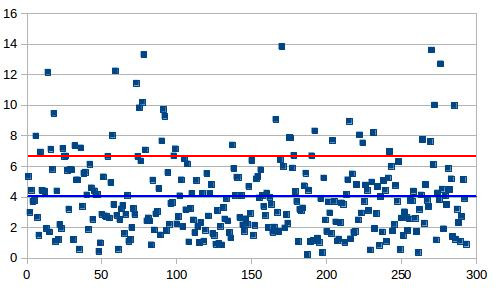
\includegraphics[height=1.7in]{images/lm1_cnn_2.jpg}}
	\caption{\footnotesize{The distribution of the distances on the first landmark. The blue line is the average value, the red line is standard deviation value.}}
	\label{figchartlm1}
\end{figure}

Figure \ref{figchart} shows the proportion of acceptable landmarks, i.e a predicted landmark is acceptable if the distance between it and the corresponding manual one is less than the average distance plus the standard deviation  value. Most of the landmarks have been detected with an accuracy greater than $75\%$. 

In the image processing point of view, the distance in $4$ pixels ($1^{st}$ landmark) is still high, it could be considered as not enough precise. Morever, when we consider the distribution of the distance in the $1^{st}$ landmark, the percent rate of the distance less than average value is not enough good. It means that we have less the predicted landmarks closed to the manual ones as we expect (like in the case of Figure \ref{figsubrs2}). So, the next step has been decided to improve these results. 

\begin{figure}[H]
	\centerline{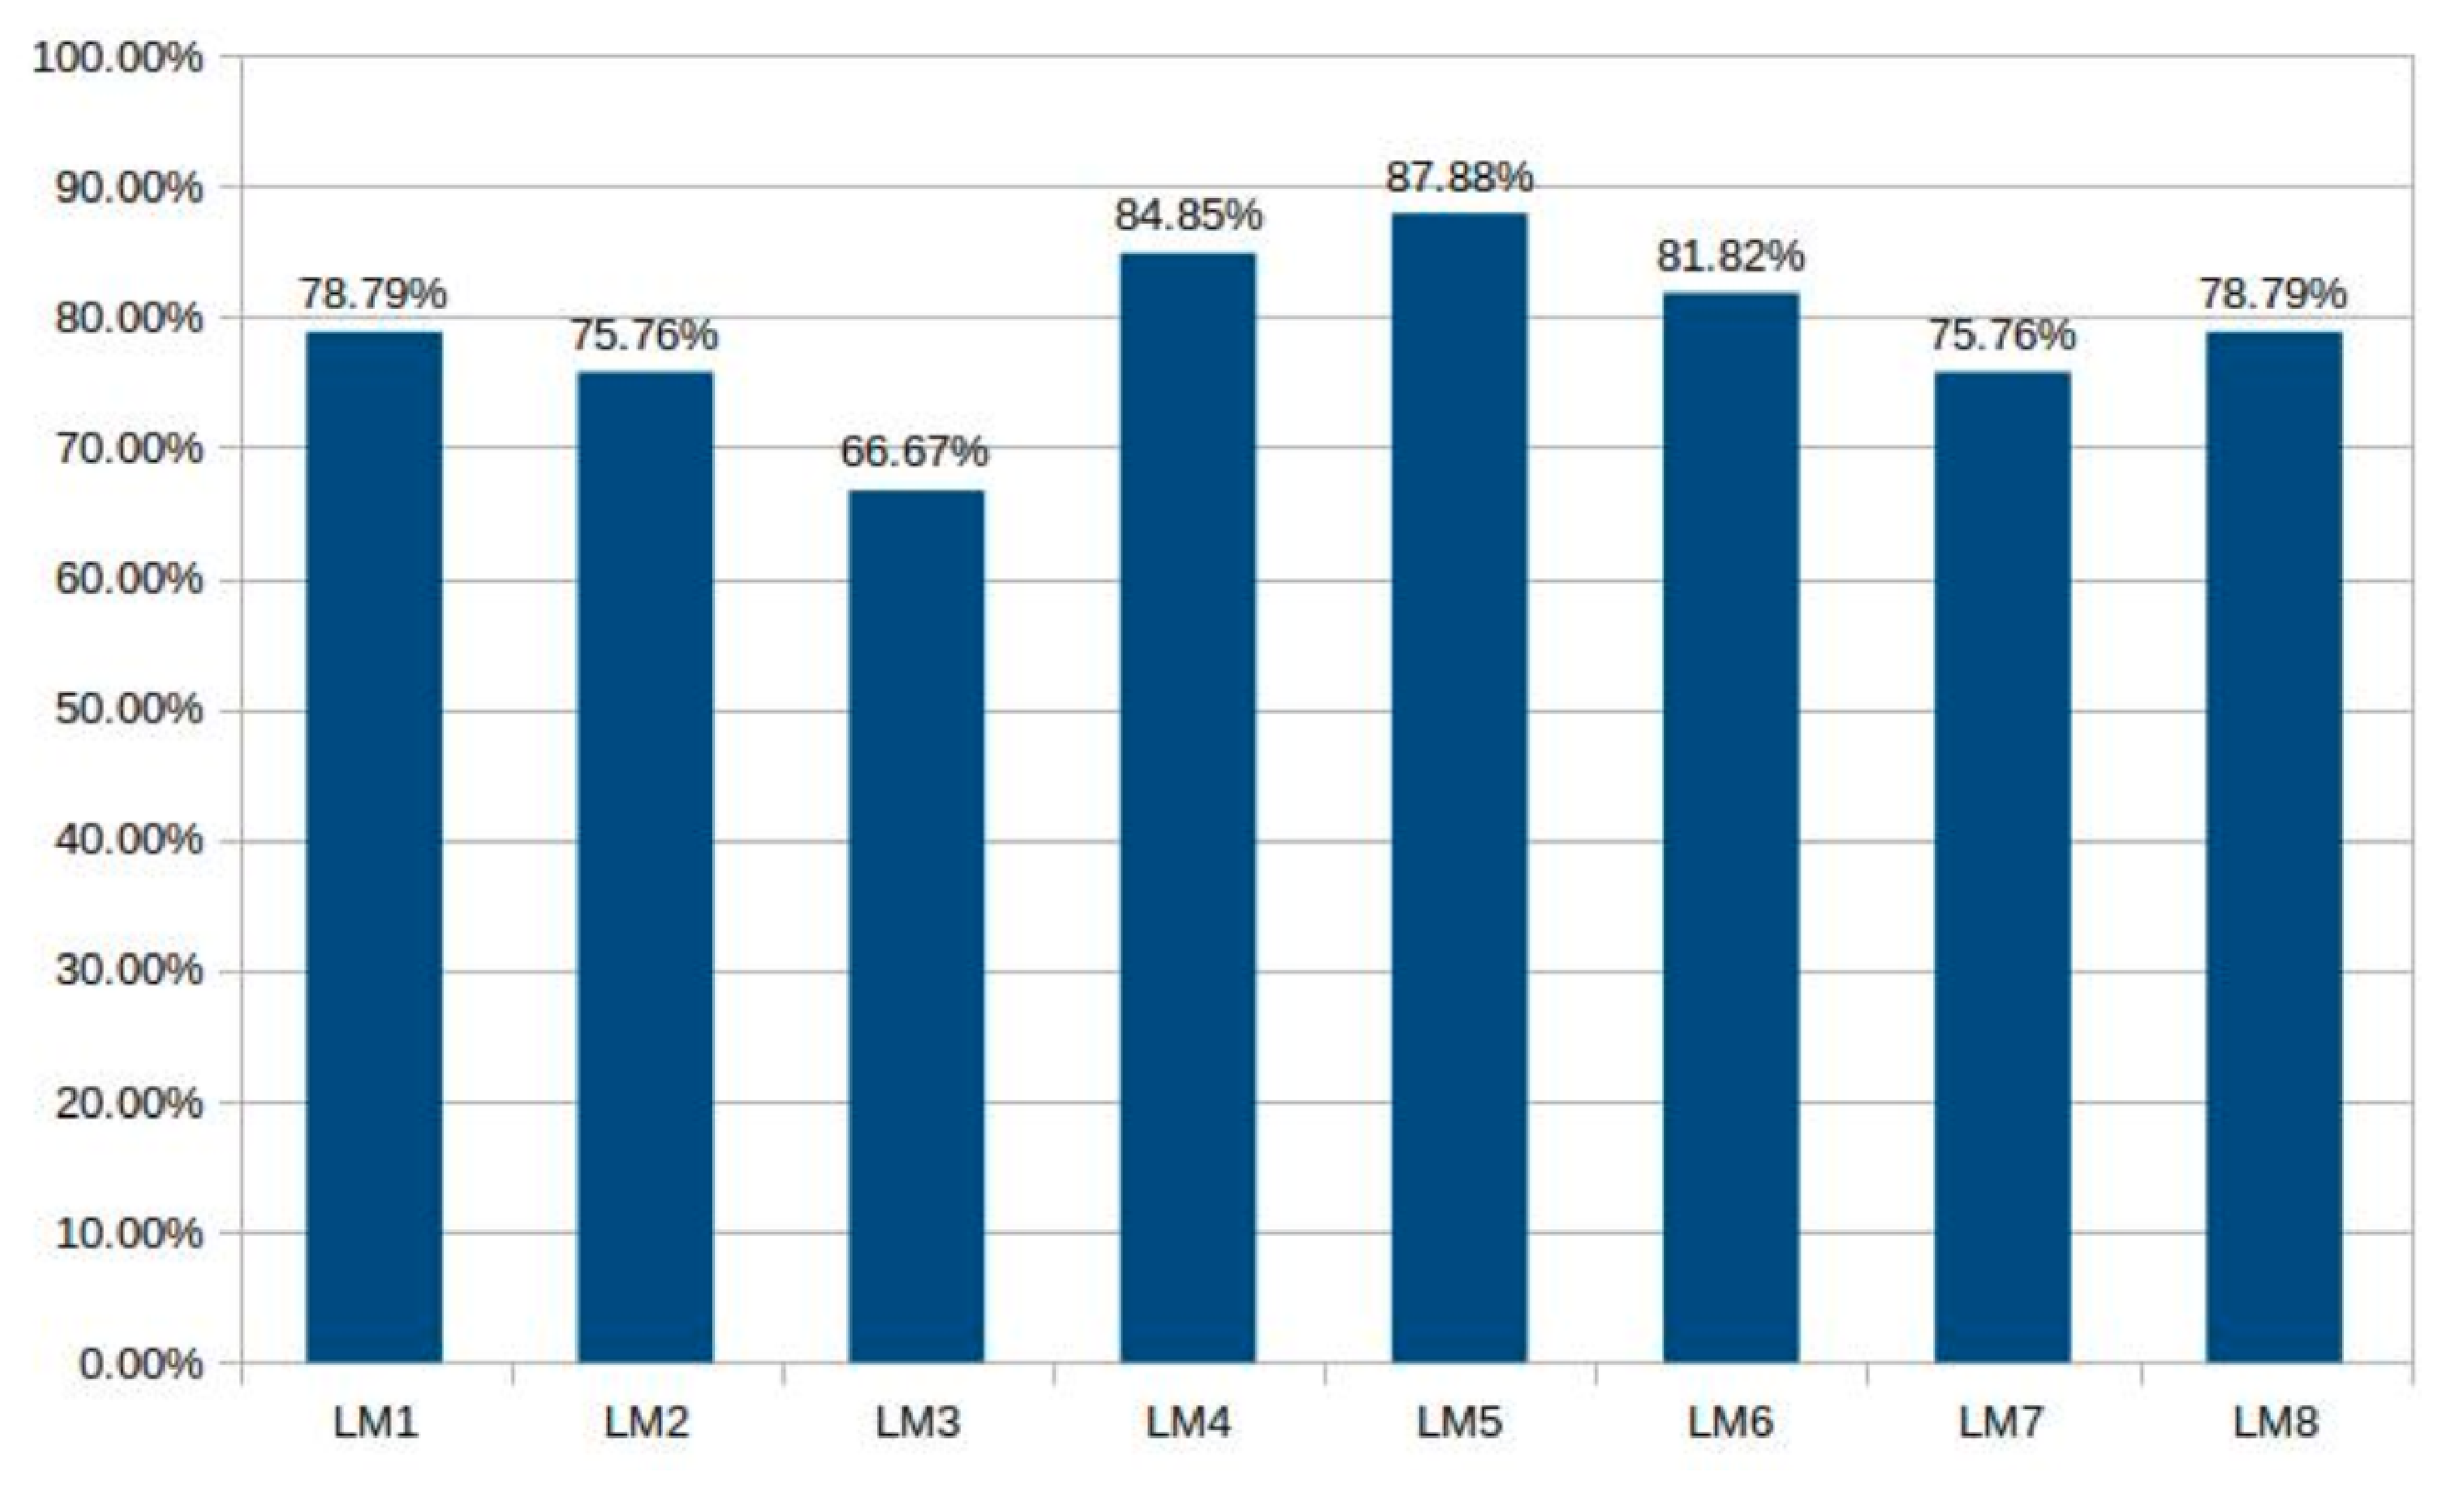
\includegraphics[height=1.8in]{images/chart.eps}}
	\caption{\footnotesize{The proportion of acceptable predicted landmarks}}
	\label{figchart}
\end{figure}

\section{Result improvement by using fine-tuning}
\label{secimproving}
As we have discussed in previous sections, the proposed network has been trained from scratch on the pronotum dataset. Even if the strengh of the correlation seems to validate the results, when the predicted landmarks are displayed on the image, the results are not enough precise since the average error is still high ($\geq 4$ pixels).

In order to reach more acceptable results for biologists, we have
broadened the model with a step of transfer learning. That is a
method that re-uses model developed for a specific task/dataset
to lead another task (called \textit{target task}) with another dataset. This allows rapid progress and improves the performance of the model on the target task \cite{torrey2009transfer}. The most popular
example has been given with the project ImageNet of Google \cite{imagenet_cvpr09} which has labeled several millions of images. The obtained parameter values which can
be used in another context to classify another dataset, eventually
very different dataset \cite{margeta2017fine}. The name of this procedure to re-use parameters
to pre-train a model is currently called \textit{fine-tuning}.

Fine-tuning does not only replace and retrain the model on the new
dataset but also fine-tunes the weights of a trained model by continuing the
backpropagation. Unfortunately, some rapid tests have shown that
re-using ImageNet features has not been relevant for our
application. We have designed a way to reproduce the method with our
own data. It is worth noting that of course the size of data to pre-train has drastically decreased. For our pre-training step, the network has been trained on the whole dataset including the images of three parts of beetle i.e pronotum, body and head. Then,
the trained model will be used to fine-tune and test on pronotum set.

\subsection{Training data preparation}
As we have mentioned, the training dataset includes a combination of the images from three
sets: pronotum, body, and head (Figure \ref{figshape3parts}). For each
set, $260$ original images have been chosen randomly for training and
validation. By applying the same procedure in section \ref{Secdataaug},
the training dataset was enlarged to $5,460$ images ($260 \times 7
\times 3$). However, the number of manual landmarks on each part is
different: \textit{$8$ landmarks on pronotum part, $11$ landmarks on
  body part, and $10$ landmarks on head part} (Figure \ref{figshape3parts}). The manual landmarks
have a specific meaning for the biologists. So, we cannot insert the
landmarks arbitrary. Instead of to do that, we keep the smallest number of
landmarks among the three parts and remove the supernumerary when it is needed. Specifically, we have removed three landmarks on the body part
($1^{st}; 6^{t}h; 9^{th}$) and two landmarks on the head part ($5{th};
6^{th}$) (Figure \ref{figshape3parts}).

\begin{figure}[H]
        \centering
        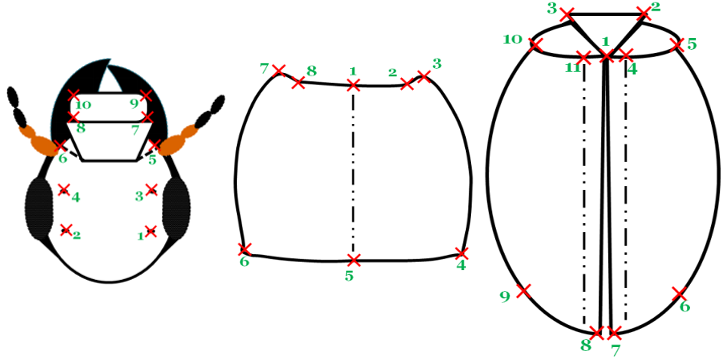
\includegraphics[height=1.6in]{images/merge.png}
    \caption{\footnotesize{A presentation of head, pronotum and body part with corresponding manual landmarks}} 
    \label{figshape3parts}
\end{figure}

\subsection{Using fine-tuning for pronotum dataset}
At the first step, the network is trained with $5,460$ images following
the same way as previously. After that, 
this trained model is used to fine-tune the pronotum dataset. To compare the result with the previous one (training from scratch), the trained model has been fine-tuned on pronotum images with different cross-validation. 

At the end of test stage, landmarks are predicted on all images in pronotum dataset. The average distances have been computed again. Table \ref{table3} shows a comparison of average distance values and standard deviation values from two studying processes: with and without fine-tuning. The \textbf{Average} \textit{from scratch} column reminds
the average distance obtained previously. The \textbf{Average} \textit{with fine-tuning}
column presents the new average distance
after fine-tuning the pronotum from the trained model. Besides, the standard errors of both cases have been presented (SD columns). It is
clearly shown that the result of predicted landmarks with the help of
fine-tuning is more precise than the first way to do it. For example, if we consider the $1^{st}$ landmarks, the average have been decreased from \textbf{$4.002$} to \textbf{$2.486$} (app. $40\%$) and the SD value have been decreased also. Even the worst average distance with fine-tuning ($3.0492$ pixels at the $6^{th}$ landmark) is still smaller than the best case with training from scratch ($4.002$ pixels at the $1^{st}$ landmark).

\begin{table}[H]
\centering
\begin{tabular}{ | c | c | c | c | c | }
\hline
	\multicolumn{1}{|c|}{\multirow{2}{*}{Landmark}} & \multicolumn{2}{c|}{From scratch} &  \multicolumn{2}{c|}{With fine-tuning}  \\ \cline{2-5}
	 & Average & SD & Average & SD \  \\ \hline
	\textbf{LM1} & \textbf{4.002} & \textbf{2.5732} & \textbf{2.486} & \textbf{1.5448} \\ \hline
	LM2 & 4.4831 & 2.7583 & 2.7198 & 1.7822 \\ \hline
	LM3 & 4.2959 & 2.7067 & 2.6523 & 1.8386 \\ \hline
	LM4 & 4.3865 & 3.0563 & 2.7709 & 1.9483 \\ \hline
	LM5 & 4.2925 & 2.9086 & 2.4872 & 1.6235 \\ \hline
	\textbf{LM6} & \textbf{5.3631} & \textbf{3.4234} & \textbf{3.0492} & \textbf{1.991} \\ \hline
	LM7 & 4.636 & 2.8426 & 2.6836 & 1.7781 \\ \hline
	LM8 & 4.9363 & 3.0801 & 2.8709 & 1.9662 \\ \hline
\end{tabular}
\caption{\footnotesize{A comparing between the average error distances, the standard deviation values per landmark of two steps.}}
\label{table3}
\end{table}

To illustrate the final results, we display the distribution of the
distance of both the best and the worst results (resp. landmark $1$
and $6$). The Figure \ref{figrsexample2} shows in (a) and (b) diagrams
 how much the average distances (blue lines) and standard errors (red lines) have
 been improved for the landmark $1$, the (c) and (d) diagrams for the
 landmark $6$. The \textit{x} and \textit{y} axes are the number of images and distance in pixels, respectively. Each point in diagram presents to the distance between predicted and corresponding manual landmark. We can see both in the best and the worst cases, the distances have been decreased and the errors have been reduced with fine-tuning.

\begin{figure}[H]
   
    \begin{subfigure}[t]{0.24\textwidth}
        \centering
        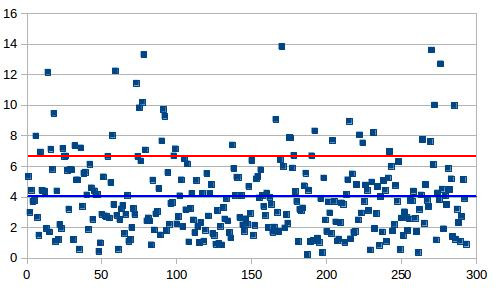
\includegraphics[height=0.9in]{images/lm1_cnn_2}
        \caption{\footnotesize{Landmark 1 - CNN}}
        \label{figsub11}
    \end{subfigure}%
    ~ 
    \begin{subfigure}[t]{0.24\textwidth}
        \centering
        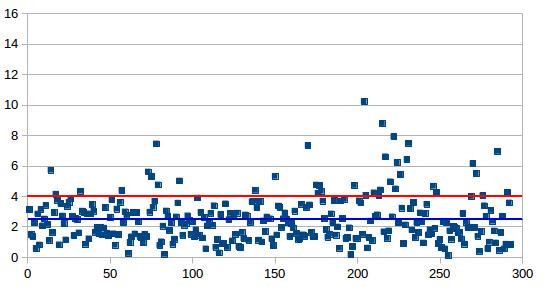
\includegraphics[height=0.9in]{images/lm1_finetuning_2}
        \caption{\footnotesize{Landmark 1 - fine-tuning}}
        \label{figsub22}
    \end{subfigure}~\\
    \begin{subfigure}[t]{0.24\textwidth}
        \centering
        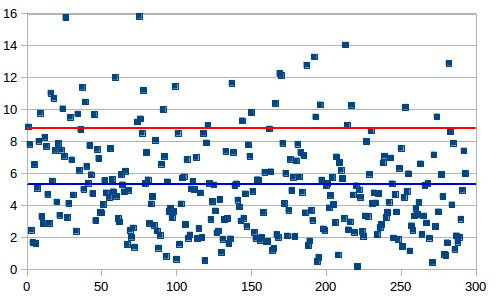
\includegraphics[height=0.9in]{images/lm6_cnn_2}
        \caption{\footnotesize{Landmark 6 - CNN}}
        \label{figsub111}
    \end{subfigure}%
    ~ 
    \begin{subfigure}[t]{0.24\textwidth}
        \centering
        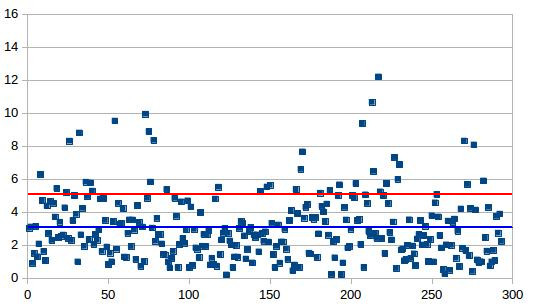
\includegraphics[height=0.9in]{images/lm6_finetuning_2}
        \caption{\footnotesize{Landmark 6 - fine-tuning}}
        \label{figsub222}
    \end{subfigure}
    \caption{\footnotesize{The distribution of distance error on $1^{st}$ and $6^{th}$ landmarks of all images in two testing steps (CNN and fine-tuning). The blue and red lines present the average distances and standard deviation values, respectively.}}
    \label{figrsexample2}
\end{figure}

As result files, the program outputs the
predicted landmarks of the images as TPS files (a standard file format for morphometric analysis softwares). With the outputs as TPS files,
the user can use MAELab framework\footnote{MAELab is a free software written in C++. It can be directly and freely
obtained by request at the authors.} to display the
landmarks on the images.

\section{Conclusion}
\label{Secconclusion}
In the context of collaboration with biologists, the project towards replacing the manual landmarks task by automatic ones on beetle's pronotum images. The pronotum images are difficult to segment, so methods which are not supposed to be based on segmentation are necessary. In this paper, after testing several models, we have presented a convolutional neural network for automatic detection landmarks on this case. It includes three times repeated structure of \textit{``elementary block"} which consists of a convolutional layer, a max pooling layer, and a dropout layer, followed by the connected layers. During the training stage, suitable techniques are used to prevent overfitting, a common issue of the neural networks. The network was trained several times in different selections of training data. After training with the manual landmarks given by the biologist, the network is able to predict the landmarks on the set of unseen images.

In our case, the training dataset is limited. So, we have applied some techniques to augment the dataset. The results from the test set have been evaluated by calculating the distance between manual landmarks and corresponding predicted-landmarks. The average of distance errors on each landmark has been also considered. Additional, a statistic on acceptable predicted landmarks has been computed with an accuracy greater than $75\%$. In order to improve the results, the model has been trained on a dataset including the images of all three parts of beetles. Then, the trained model has been used to fine-tune and to test on pronotum images.

These results have shown that using the convolutional network to predict the
landmarks on biological images leads to satisfying results without need for segmentation step on the object of interest. The
best set of estimated landmarks has been obtained after a step
of fine-tuning using the whole set of images that we have for the
project, i.e. about all beetle parts. The quality of prediction allows using automatic landmarking to replace manual landmarks. 

Currently, we are applying the network on other parts of beetle, i.e. head and elytra part and the results seem to be good also. Besides, after finding that the well-known pretrained model do not accord to our problem, the next step is to study more deeply how to characterize the learning problem to design the right pretrained model depending the class of the problem.

\paragraph{Acknowledgment}

The research has been supported by DevMAP project\footnote{https://www6.rennes.inra.fr/igepp\_eng/Research\-teams/Demecology/Projects/INRA\-SPE\-DevMAP}. We would like to thank our colleague, ALEXIA Marie, who have provided manual landmarks on beetle images.

\footnotesize{

\bibliographystyle{plain}
\bibliography{includes/references}

} 

\end{multicols}

\end{document}

\begin{thebibliography}{99}

\end{thebibliography}{90}

torrey2009transfer
imagenet_cvpr09
margeta_mri








\begin{thebibliography}{99}
\bibitem{journal1}
	M. Uzunoglu, M. S. Alam, ``Dynamic modeling, design, and simulation of a combined PEM fuel cell and ultracapacitor system for stand-alone residential applications" IEEE Trans. Ener. Conv., \textbf{21}(3), 767--775, 2006. https://doi.org/10.1109/TEC.2006.875468


\hspace{-1cm} \textbf{Conference Papers:}

\bibitem{conf1} 
S. Mumtaz, L. Khan, ``Performance of Grid-Integrated Photovoltaic/Fuel Cell/ Electrolyzer/Battery Hybrid Power System" in 2nd International Conference on Power Generation Systems and Renewable Energy Technologies, Islamabad Pakistan, 2015. https://doi.org/10.1109/PGSRET.2015.7312249

\hspace{-1cm} \textbf{Thesis:}

\bibitem{thesis} 
	H. Lihua, ``Analysis of Fuel Cell Generation System Application", Ph.D Thesis, Chongqing University, 2005.

\hspace{-1cm} \textbf{Books:}

\bibitem{book1} 
	X. Li, Principles of Fuel Cells, Taylor and Francis Group, 2006.

\bibitem{book2} 
	M. H. Nehrir, C. Wang, Modeling and Control of Fuel Cells: Distributed Generation Applications, Wiley-IEEE Press, 2009.

%\end{enumerate}
\end{thebibliography}{90}